%-*- TeX -*- -*- Soft -*-,
% http://www.gigasciencejournal.com/authors/instructions/commentary 

\documentclass[11pt]{bmc_article_s50}

\usepackage{amsthm,amsmath}
\usepackage{siunitx}
\usepackage[colorinlistoftodos]{todonotes}
\usepackage[utf8]{inputenc}
\RequirePackage{hyperref}
\usepackage{array}
\newcolumntype{L}[1]{>{\raggedright\let\newline\\\arraybackslash\hspace{0pt}}p{#1}}
\newcolumntype{R}[1]{>{\raggedleft\let\newline\\\arraybackslash\hspace{0pt}}p{#1}}
\usepackage{longtable}
\usepackage{booktabs}
\usepackage{url}
\urlstyle{rm}
\usepackage{setspace}
\usepackage[T1]{fontenc}
\pagestyle{empty}
\setlength{\parindent}{0cm}
\usepackage{ragged2e}
\justifying
\singlespace

\begin{document} % (800-1200 words)

\title{Brainhack: A collaborative workshop for the open neuroscience community}
\maketitle
\author[1,2*]{R Cameron Craddock}\cor{}\email{ccraddock@nki.rfmh.org}
\author[3]{Pierre Bellec}\email{pierre.bellec@criugm.qc.ca}
\author[4]{Daniel S Margulies}\email{margulies@cbs.mpg.de}
\author[4]{B Nolan Nichols}\email{nolan.nichols@gmail.com}

\address[1]{
  Computational Neuroimaging Lab, Center for Biomedical Imaging and \\\hspace*{59pt}Neuromodulation, Nathan S. Kline Institute for Psychiatric Research, \\\hspace*{59pt}140 Old Orangeburg Rd, 10962, Orangeburg, New York, USA
}
\address[2]{
  Center for the Developing Brain, Child Mind Institute, 445 Park Ave,\\\hspace*{59pt} 10022, New York, New York, USA
}
\address[3]{Centre de recherche de l’institut de g\'{e}riatrie de   Montr\'{e}al, Montr\'{e}al, QC, Canada
}
\address[4]{
  Max Planck Research Group for Neuroanatomy \& Connectivity,\\\hspace*{59pt} Max Planck Institute for Human Cognitive and Brain Sciences, \\\hspace*{59pt} Stephanstraße 1A, 04103, Leipzig, Germany
}
\address[5]{
  SRI International, 333 Ravenswood Ave, 94025, Menlo Park,  California, USA
}
\address[6]{
  Department of Psychiatry and Behavioral Sciences, Stanford University,\\\hspace*{59pt} 
  1265 Welch Road, 94306, Stanford,  California, USA
}


\begin{abstract} % (max 100 words)
Brainhack events bring together 

\end{abstract}

\keywords{hackathon, unconference, open science, neuroscience, data sharing, collaboration}

\section{Introducing Brainhack}

Now in their fifth year, international and regional Brainhack events bring together brain enthusiasts from a variety of backgrounds to build relationships, learn from one another, and collaborate on projects related to the neurosciences. Brainhacks are unconventional events that adapt concepts from both ``hackathons'' and ``unconferences'' to engage in topics related to brain research. Similar to hackathons, Brainhack events primarily involve unstructured time during which participants collaborate intensively to initiate, develop, and complete various projects. Rather than focusing on computer programming, projects at Brainhacks can be completed using a much broader array of methods. Time is also set aside for periodic unconference sessions, which involve presentations whose content is dynamically determined based on the interests of attendees. In consideration of the ever expanding interest in the tools of open science, Brainhack has developed an eductional component that runs in parallel to the hacking sessions in order to introduce the basic tools of open collaboration. This combined model encourages active participation and interaction between attendees, while also maximizing the topical relevance of the more formally presented content (see Figure~\ref{fig1}).

\begin{figure}[htp]
\begin{center}
  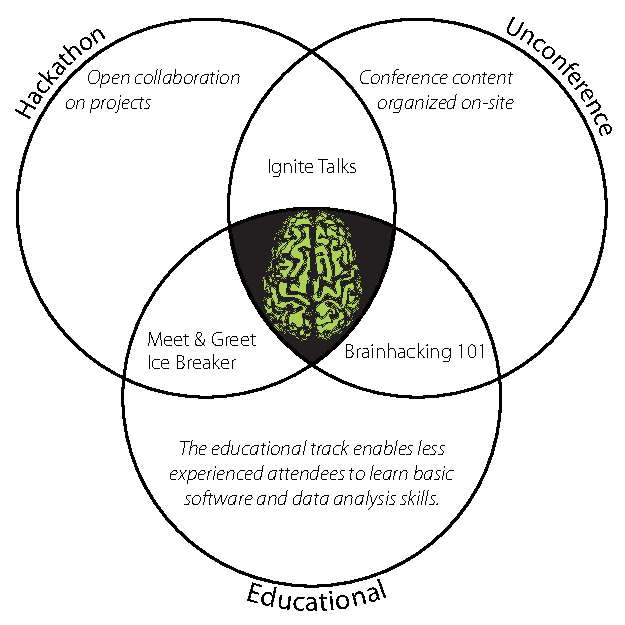
\includegraphics[width=0.5\textwidth]{Figure_01}
  \caption{\href{http://www.brainhack.org}{Brainhack} is composed of various organizational features from ``unconferences'' and ``hackathons'', and includes a variety of scheduling components to encourage collaboration and introduction to open science methods.}
  \label{fig1}
\end{center}
\end{figure}

There is no ideal background, skill set, or experience level required for Brainhack attendees. Fully translating neuroscience data to knowledge requires expertise that spans the gamut from biology, computer science, engineering, informatics, mathematics, neuroanatomy, philosophy, physics, psychiatry, psychology, statistics, art, and many others. The goal of a Brainhack event is to facilitate the cross pollination of ideas and knowledge across these various disciplines and communities and to accelerate the development of a richer understanding of the brain. In addition to sharing data and tools, attendees can contribute in a variety of ways. Philosophical debates about the meanings of cognition, coordinated efforts to manually segment brain images from different species, curating neuroscience literature, or helping others to understand the subtleties of diagnosing a developmental disorder are all examples of valuable contributions that have emerged at Brainhacks (for further examples, see Table~\ref{tab3}).

\section{Hackathons based on collaboration, not competition}

The hackathon format gained prominence in the technology sector by providing a meeting model that targets specific project goals during intense time-limited collaborations. The competitive aspect of the traditional hackathon, while catalyzing rapid advances toward specific technology ends, is contrary to the founding motive of Brainhack, which is to encourage open, cross-institutional and inter-disciplinary collaboration. Rather than subdividing attendees into competitive factions, Brainhack attendees are encouraged to work together in collaborative teams to solve problems of their choosing. In this way, rather than obtaining many solutions to a single problem, we aim to produce various solutions to many problems. Most importantly, we encourage the building of new relationships that continue to be productive beyond the end of the event.

\subsection{Brainhack projects}

Rather than focusing on a specific problem or toolset, which is common at more standard Hackathons, attendees are encouraged to generate their own projects ideas around which they can self-assemble into project teams. As a consequence, some projects may receive more limited interest, whereas another might attract the majority of attendees. In this way, the projects developed at Brainhacks are elected by participation, rather than being pre-specified by the event organizers. This model is more conducive to collaboration than the alternative model of organizing a Hackathon around a challenge or competition. While there are of many different alternative models between these two extremes, we are currently working on building thematic Brainhack events that bring researchers together to focus on more specific questions in neuroscience.

To date, projects that have been completed at Brainhack events have spanned from students interacting with more experienced researchers to learn about a new data modality or analysis method, inter-disciplinary collaborations to improve data collection for hyper-kinetic populations, the development or optimization of data analysis tools, to testing hypothesis about brain structure using openly shared data. See Table~\ref{tab3} for selected examples of projects that have previously been initiated at Brainhack events, and \href{http://www.brainhack.org}{www.brainhack.org} for a full list of projects.

\subsection{Event organization}

Brainhack events span one to four days and included a variety of content to make them accessible and fruitful for a wide range of attendees. The format of the events is not fixed, but varies based on the needs determined by the local organizing committee. At past events, the schedule has included various components aiming to quickly integrate the attendees and generate an environment condusive to productive collaboration. We have found the activity categories included in Table~\ref{tab4} to be valuable components of creating a productive environment. 

Considering the novel format of such events, the attendance fees are kept as low as possible to encourage attendence. This has been made possible in the past through generous financial support and meeting space from local hosting institutions and corporate sponsors. When possible, lunch and dinner have been provided to encourage continued interaction between attendees throughout the duration of the event. We have also aimed to reduce travel costs by co-locating events with other international workshops, such as the 2012 Resting Workshop in Magdeburg Germany, and annual meetings of the Organization of Human Brain Mapping (OHBM). OHBM has been particularly supportive of the Brainhack model and the annual OHBM Hackathon has evolved to include a two-day intensive hackathon, an additional educational day that is open to all OHBM attendees, and an open collaboration room that is available throughout the meeting.

\subsubsection{Distributed events}

The Brainhack began as international events that drew attendees from all over the world to work together in open collaboration. Initial efforts to transfer this model to the local level were less successful due to fears that local events would not be able to provide enough content to attract attendees. Brainhack Eastern Daylight Time (Brainhack EDT) was developed to address these concerns by organizing several simultaneous events and linking them together to share content. Events were limited to sites in time zones within one hour of eastern daylight time to simplify scheduling. This innovative distributed model drew 150 attendees across seven sites located in three different countries, and has since been followed by Brainhack Americas, which extended this model to the entirety of North, South and Central America (see Tables \ref{tab1} and \ref{tab2}).

\subsection{Post-conference publications}

motivate post-conference publications and brainhack thematic series

\section{Conclusions}

Considering the relative novelty of the Brainhack event, there remains substantial space of innovative programming components and improvement in structure. With the general aim of building a productive working conference, ...

Further development of infrastructure for distributed Brainhack events to facilitate local hosting of events. 

Finally, the educational component encourages future participation and provides the tools ...

%%%%%%%%%%%%%%%%%%%%%%%% END MATERIAL %%%%%%%%%%%%%%%%%%%%%%%
%\theendnotes
\newpage
\section*{Availability of Supporting Data}
More information about Brainhack, including projects from past and future events, can be found at~\href{http://www.brainhack.org}{www.brainhack.org}.

\section*{Competing interests}
None

\section*{Author's contributions}
RCC, PB, DSM, and BNN wrote the manuscript.

\section*{Acknowledgements}
The authors would like to thank prior attendees of Brainhacks over the past fours years in Leipzig, Paris, etc... \todo{add content. include list of sponsors?}

%%%%%%%%%%%%%%%%%%%%%%%%%%% TABLES %%%%%%%%%%%%%%%%%%%%%%%%%%
\begin{table}[!ht]
\caption{{\bf Selected examples of Brainhack projects}\label{tab3}}
\hrule %\hline
    \begin{itemize}
    \item 
        A child psychiatrist and a 3D video artist initiated a collaboration at the 2012 Brainhack to develop a movie to be shown to participants during resting-state fMRI scans to reduce head motion in hyperkinetic populations \cite{inscapes, vanderwal2015}.
    \item 
        The ABIDE Preprocessing Initiative \cite{abide_preproc} is an ongoing project started at the 2012 Brainhack to share preprocessed versions of the Autism Brain Imaging Data Exchange (ABIDE) dataset \cite{abide, dimartino2014}. This project is sharing functional data that have been processed using the Connectome Computation System (CCS) \cite{ccs, Xu2015}, the Configurable Pipeline for the Analysis of Connectomes (C-PAC) \cite{cpac, craddock2013}, the Data Preprocessing Assistant for Resting State fMRI (DPARSF) \cite{dparsf, yan2010}, and the Neuro Imaging Analysis Kit (NIAK) \cite{niak, bellec2011}, as well as cortical thickness measures extracted from structural data using FreeSurfer \cite{freesurfer, fischl2000}, CIVET \cite{civet, zijdenbos2002}, and Advanced Normalization Tools (ANTS) \cite{ants, tustison2014}.
    \item
        A collaboration started at the 2012 Brainhack performed an analysis to identify differences in cortical thickness and structural covariance between individuals with autism spectrum disorder and neurotypical controls \cite{Valk2015}.
    \item
        A project team at Brainhack 2013 amassed a dataset of 14,781 structural MRI scans to estimate the distribution of brain sizes across individuals for optimizing scan acquisition parameters \cite{Mennes2014}.
    \item 
        The development team of LORIS, an open source database system for neuroimaging and phenotypic data, have repeatedly used Brainhack as an opportunity to meet and collaborate on new features \cite{Das2012}.
    \item
        An early version of the Daydreaming app \cite{dayapp}, an Android application for real-time assessment of users' mind-wandering, was developed at Brainhack 2013.
    \item 
        The Clubs of Science \cite{clubs} project, founded at Brainhack MTL 2015, has built a web-based visualization of the social web underlying neuroimaging research.
    \item
        The linkRbrain \cite{linkrbrain} tool for integrating and querying neuroimaging data with activation peaks from the literature and gene expression data  was partially developed and first tested at Brainhack 2013 in Paris \cite{Mesmoudi2015}. 
    \end{itemize}
\hrule %\hline
\smallskip Further projects can be found at www.brainhack.org \cite{brainhackorg}.
\end{table}

\begin{table}[!ht]
\caption{{\bf Brainhack events occurring 2012 - 2013.} The number of attendees for each event are included in parenthesis. $^\star$Local organizers for an event. $^\dagger$Distributed event main organizer.}\label{tab1}
  \begin{tabular}{L{.1in}L{.1in}L{2.4in}L{2in}L{1.5in}}
    \hline
  \\
    \multicolumn{3}{l}{\textbf{2012 Brainhack and Unconference}} &  & September 1 - 4, 2013  \\
  & \multicolumn{3}{l}{Leipzig, Germany (77)} \\
    & & \multicolumn{3}{l}{Host: Max Planck Institute for Human Cognition and Brain Sciences} \\
    & & \multicolumn{3}{l}{Organizers: Daniel Margulies$^{\star}$, Pierre Bellec, Cameron Craddock, Donald McLaren,} \\
    & & \multicolumn{3}{l}{\hspace*{25pt}Maarten Mennes}\\
  \\
  \multicolumn{3}{l}{\textbf{OHBM Hackathon 2013}} & & June 16 - 20, 2015  \\
   & \multicolumn{3}{l}{Seattle, Washington, USA (136)} \\
   & & \multicolumn{3}{l}{Host: Organization for Human Brain Mapping } \\
   & & \multicolumn{3}{l}{Organizers: Nolan Nichols$^{\star}$, Tom Grabowski, Chinh Dang, Elaine Shen,} \\
   & & \multicolumn{3}{l}{\hspace*{25pt}Rachel Pizarro, Jamie Kinney, Satra Ghosh} \\
   \\
    \multicolumn{3}{l}{\textbf{Brainhack 2013}} & & October 23 - 26, 2013  \\
  & \multicolumn{3}{l}{Paris, France (77)} \\
    & & \multicolumn{3}{l}{Host: Laboratoire d'Imagerie Biom\'{e}dicale, Sorbonne Universit\'{e}s, Universit\'{e} Pierre-et- } \\
    & & \multicolumn{3}{l}{\hspace*{25pt}Marie-Curie, Paris 06, CNRS, INSERM} \\
    & & \multicolumn{3}{l}{Organizers: Selma Mesmoudi$^{\star}$, Yves Burnod$^{\star}$, Donald McLaren, Cameron Craddock,} \\
    & & \multicolumn{3}{l}{\hspace*{25pt}Pierre Bellec, Daniel Margulies, Maarten Mennes} \\
  \\
    \multicolumn{3}{l}{\textbf{OHBM Hackathon 2014}} & & July 5 - 7, 2014  \\
  & \multicolumn{3}{l}{Berlin, Germany (77)} \\
    & & \multicolumn{3}{l}{Host: Organization for Human Brain Mapping } \\
    & & \multicolumn{3}{l}{Organizers: Daniel Margulies$^{\star}$, Pierre Bellec, Cameron Craddock, Tom Grabowski,} \\
    & & \multicolumn{3}{l}{\hspace*{25pt}Sean Hill, Nolan Nichols, JB Poline} \\
  \\
    \multicolumn{3}{l}{\textbf{Brainhack Eastern Daylight Time}} & & October 18 - 19, 2014  \\
    & \multicolumn{3}{l}{Ann Arbor, Michigan, USA (77)} \\
    & & \multicolumn{3}{l}{Host: University of Michigan } \\
    & & \multicolumn{3}{l}{Organizers: Scott Peltier$^{\star}$, Robert Welsh$^{\star}$} \\
    & \multicolumn{3}{l}{Boston, Massachusetts, USA (77)} \\
    & & \multicolumn{3}{l}{Host: Massachusetts Institute of Technology} \\
    & & \multicolumn{3}{l}{Organizers: Satra Gosh$^{\star}$, Matt Hutchison$^{\star}$, Donald McLaren$^{\star}$} \\
    & \multicolumn{3}{l}{Miami, Florida, USA (77)} \\
    & & \multicolumn{3}{l}{Host: Florida International University} \\
    & & \multicolumn{3}{l}{Organizers: Angie Laird$^{\star}$, Lucina Uddin$^{\star}$} \\
    & \multicolumn{3}{l}{Montr\'eal, Qu\'ebec, Canada (77)} \\
    & & \multicolumn{3}{l}{Host: Centre de recherche de l'Institut universitaire de g\'{e}riatrie de Montr\'{e}al} \\
    & & \multicolumn{3}{l}{Organizers: Benjamin De Leener$^{\star}$, Julien Cohen-Adad$^{\star}$, Pierre Bellec$^{\star}$} \\
    & \multicolumn{3}{l}{New York, New York, USA (77)} \\
    & & \multicolumn{3}{l}{Host: Child Mind Institute and Columbia University} \\
    & & \multicolumn{3}{l}{Organizers: Cameron Craddock$^{\star\dagger}$, Andrew Gerber$^{\star}$} \\
    & \multicolumn{3}{l}{Porto Alegre, Brazil (77)} \\
    & & \multicolumn{3}{l}{Host: Pontif\'{i}cia Universidade Cat\'{o}lica do Rio Grande do Sul} \\
    & & \multicolumn{3}{l}{Organizers: Alex Franco$^{\star}$, Caroline Fr\"{o}hlich$^{\star}$, Felipe Meneguzzi$^{\star}$} \\
    & \multicolumn{3}{l}{Toronto, Ontario, Canada (77)} \\
    & & \multicolumn{3}{l}{Host: University of Toronto} \\
    & & \multicolumn{3}{l}{Organizers: Jonathan Downer$^{\star}$, Katie Dunlop $^{\star}$, Stephen Strother$^{\star}$} \\
    & \multicolumn{3}{l}{Washington DC, USA (77)} \\
    & & \multicolumn{3}{l}{Host: Georgetown University} \\
    & & \multicolumn{3}{l}{Organizers: John Van Meter$^{\star}$, Lei Liew$^{\star}$, Ziad Saad$^{\star}$, Prantik Kundu$^{\star}$} \\
  \\
  \hline
  \end{tabular}
\end{table}

\begin{table}[!ht]
\caption{{\bf Brainhack events in 2015.} The number of attendees for each event are included in parenthesis. $^\star$Local organizers for an event. $^\dagger$Distributed event main organizer.}\label{tab2}
  \begin{tabular}{L{.1in}L{.1in}L{2.4in}L{2in}L{1.5in}}
    \hline
  \\
    \multicolumn{3}{l}{\textbf{OHBM Hackathon 2015}} & & June 12 - 14, 2015  \\
  & \multicolumn{3}{l}{Honolulu, Hawaii, USA (59)} \\
    & & \multicolumn{3}{l}{Host: Organization for Human Brain Mapping } \\
    & & \multicolumn{3}{l}{Organizers: Nolan Nichols$^{\star}$, Pierre Bellec, Cameron Craddock, Tom Grabowski,} \\
    & & \multicolumn{3}{l}{\hspace*{25pt}Jack Van Horn, Daniel Margulies, JB Poline, and the OHBM 2015 Local Organizing Committee} \\
  \\
    \multicolumn{3}{l}{\textbf{Brainhack Montreal 2015}} & & July 27 - 29, 2015 \\
  & \multicolumn{3}{l}{Montr\'{e}al, Qu\'{e}bec, Canada (53)} \\
    & & \multicolumn{3}{l}{Host: Centre de recherche de l'Institut universitaire de g\'{e}riatrie de Montr\'{e}al} \\
    & & \multicolumn{3}{l}{Organizers: Benjamin De Leener$^{\star}$, Julien Cohen-Adad$^{\star}$, Pierre Bellec$^{\star}$} \\
    & & \multicolumn{3}{l}{\hspace*{25pt}Sebastien Dery$^{\star}$, Pierre-Olivier Quirion$^{\star}$} \\
  \\
    \multicolumn{3}{l}{\textbf{Brainhack Americas}} & & October 23 - 25, 2015  \\
    & \multicolumn{3}{l}{Ann Arbor, Michigan, USA (10)} \\
    & & \multicolumn{3}{l}{Host: University of Michigan } \\
    & & \multicolumn{3}{l}{Organizers: Scott Peltier$^{\star}$, Robert Welsh$^{\star}$} \\
  
    & \multicolumn{3}{l}{Berkeley, California, USA (7)} \\
    & & \multicolumn{3}{l}{Host: D-Lab, University of California, Berkeley} \\
    & & \multicolumn{3}{l}{Organizers: Daniel Lurie$^{\star}$, JB Poline$^{\star}$} \\
  
    & \multicolumn{3}{l}{Los Angeles, California, USA (38)} \\
    & & \multicolumn{3}{l}{Host: University of Southern California} \\
    & & \multicolumn{3}{l}{Organizers: Lei Liew$^{\star}$, Gautam Prasad$^{\star}$, Yonggang Shi$^{\star}$} \\
  
    & \multicolumn{3}{l}{Miami, Florida, USA (50)} \\
    & & \multicolumn{3}{l}{Host: University of Miami} \\
    & & \multicolumn{3}{l}{Organizers: Lucina Uddin$^{\star}$, Angie Laird$^{\star}$}  \\
  
    & \multicolumn{3}{l}{New York, New York, USA (33)} \\
    & & \multicolumn{3}{l}{Host: Translational \& Molecular Imaging Institute, Icahn School of Medicine} \\
  & & \multicolumn{3}{l}{\hspace*{25pt}at Mount Sinai and Child Mind Institute} \\
    & & \multicolumn{3}{l}{Organizers: Christopher Cannistraci$^{\star}$, Prantik Kundu$^{\star}$, David O'Connor,} \\
  & & \multicolumn{3}{l}{\hspace*{25pt} Ting Xu, Cameron Craddock$^{\dagger}$,} \\
  
    & \multicolumn{3}{l}{Porto Alegre, Brazil (30)} \\
    & & \multicolumn{3}{l}{Host: Pontif\'{i}cia Universidade Cat\'{o}lica do Rio Grande do Sul} \\
    & & \multicolumn{3}{l}{Organizers: Alexandre Franco$^{\star}$, Anibal S\'{o}lon Heinsfeld, Felipe Meneguzzi$^{\star}$, Ramon Fraga Pereira}\\
  
    & \multicolumn{3}{l}{Quer\'{e}taro, M\'{e}xico (31)} \\
    & & \multicolumn{3}{l}{Host: Instituto De Neurobiolog\'{i}a, Universidad Nacional Aut\'{o}noma de M\'{e}xico} \\
    & & \multicolumn{3}{l}{Organizers: Sarael Alcauter$^{\star}$, Fernando Barrios$^{\star}$, Cameron Craddock$^{\dagger}$,}\\
  & & \multicolumn{3}{l}{\hspace*{25pt}Eric H Pasaye$^{\star}$} \\
  
    & \multicolumn{3}{l}{Seattle, Washington, USA (12)} \\
    & & \multicolumn{3}{l}{Host: University of Washington eScience Institute} \\
    & & \multicolumn{3}{l}{Organizers: Ariel Rokem$^{\star}$} \\
  \\
  \hline
  \end{tabular}
\end{table}

\begin{table}[!ht]
\caption{{\bf Programming components of Brainhack events.} }\label{tab4}
\hline
    \begin{itemize}
    \item
        \textbf{Meet and great:} Brainhack events begin with a welcome to the hosting facility by the local organizing committee, along with a briefing about the event schedule, procedures, or other information that might be important for the attendees.
    \item
        \textbf{Ice breaker:} Interaction between attendees is the key to a successful Brainhack event. The ice breaker is an activity to introduce attendees and their interests on one another. One strategy that has been successful is for each attendee to give their name, their institution, and three words that describe their interests. Such ice breakers could take various forms, including a speed-dating paradigm in which attendees pair-up for a brief conversation, after which attendees swap partners, and this continues until every pair has met.
    \item
        \textbf{Ignite talks:} Brainhack's equivalent of keynote sessions, Ignite talks are inspirational talks on the big picture of open brain science that are intended to invigorate the audience for the day ahead. These are ideally brief (10 minute presentation followed by 10 minutes of questions), of general relevance, and are provided by a luminary in the field.
    \item
        \textbf{Hacking:} The core of Brainhack is ``open hacking'' sessions during which attendees collaborate together on projects of their choosing. Attendees who have specific project ideas or data that they would like to explore are encouraged to advertise their project at \href{http://www.brainhack.org}{www.brainhack.org} prior to the event. On the opening of the Brainhack event, typically after the ice breaker, attendees pitch their ideas and afterwards mingle with others to organize a project team. Teams work together throughout the remainder of Brainhack and are given the opportunity to present their progress during the wrap-up session at the end of the event.
    \item
        \textbf{Brainhacking 101:} The educational track enables less experienced attendees to learn basic software and data analysis skills. Occuring in parallel so as not to interfere with the ongoing hacking sessions, this track begins with ``Installfest'' sessions during which attendees receive help installing needed software. Afterwards are several hands-on tutorials that cover topics like: using Github, Python programming, using Python to load and visualize neuroimaging data, and performing meta-analyses of scientific literature. The resources for educational sessions are made freely available online (e.g., see \href{https://github.com/ohbm/brain-hacking-101}{github.com/ohbm/brain-hacking-101}).
    \item
        \textbf{Unconference:} Sessions for attendees to present on their research or other topics of current interest. Immediately prior to these sessions, the agenda is determined on-site. Attendees who are willing to present add their name to a sign-up sheet and in the event that there are more interested presenters than time, the group is polled to determine which presentations are given time or to extend the amount of time allotted. Instead of unconference sessions, some sites have incorporated ``Data Blitzes'', consisting of preorganized session where attendees have the opportunity to present their research. Brainhack Miami has had success with this model and has secured funding to award monetary prizes to the best presentations.
    \item
        \textbf{Wrap-up and feedback:} Brainhack events typically finish with a wrap-up session during which project teams describe the progress that they made or give a demo of their results in a brief (~1-2 minute) presentation. Afterwards, the local organizers lead a discussion about what worked well with the event, and how it could be improved in the future.
    \end{itemize}
\hline
\end{table}

%%%%%%%%%%%%%%%%%%%%%%%%%%% BIBLIOGRAPHY %%%%%%%%%%%%%%%%%%%%
\bibliographystyle{bmc-mathphys} 
\bibliography{brainhack-commentary} 
\end{document}
